\documentclass[11pt]{report}
\input{../pri-end/T0_preamble_standalone_A4_De}
% T0_preamble_patches.tex — LOKALER PLATZHALTER
% Im Repo durch die offizielle Version ersetzen.

\fancyhead[L]{\small\textcolor{t0gray}{FFGFT · Rotverschiebung achromatisch}}
\fancyhead[R]{\small\textcolor{t0gray}{Johann Pascher · 2026}}
\title{Rotverschiebung in FFGFT: statisch, achromatisch\\
\large und die $z\to$Zeit-Übertragung auf das expandierende Bild\\
\large mit der kosmologischen Entartung (Dok.~267)}
\author{Johann Pascher}
\date{2026}
\begin{document}
\maketitle
\tableofcontents
\newpage
% ============================================================
% 280_T0_Rotverschiebung_Achromatisch_De_ch.tex
% Rotverschiebung in FFGFT: statisch, achromatisch, und die z->Zeit-Uebertragung
% Quellen: Dok. 064, 025/026, 063 (korrigiert), 267; Status/Korrektur: Dok. 190 (K6)
% ============================================================

\section*{Worum es geht}

In FFGFT entsteht die kosmische Rotverschiebung \emph{nicht} durch Raumexpansion,
sondern durch einen statischen geometrischen Mechanismus im $\xi$-Feld. Diese Note
hält drei Punkte fest und korrigiert einen vierten:

\begin{enumerate}
  \item \textbf{Statisch:} $1+z = e^{\xi x}$, also $z \approx \xi\,x$ -- Energieverlust
        bzw.\ fraktale Wegverlängerung entlang des Lichtwegs, kein Skalenfaktor $a(t)$
        (Dok.~064, 025/026).
  \item \textbf{Achromatisch:} Die fraktale Wegverlängerung ist rein geometrisch und
        streckt \emph{alle} Wellenlängen mit demselben Faktor -- sie ist
        \emph{nicht} wellenlängenabhängig. Finite-Elemente-Simulationen der Geometrie
        bestätigen das. (\textbf{Korrektur} der früheren chromatischen Darstellung;
        Dok.~190~K6.)
  \item \textbf{Die $z\to$Zeit-Achse ist ein $\Lambda$CDM-Konstrukt:} Weil FFGFT kein
        $a(t)$ hat, ist jede Auftragung einer Größe \enquote{über kosmische Zeit}
        (z.\,B.\ die Lilly--Madau-Sternentstehungsrate) nur eine \emph{Übertragung
        der Beobachtung auf das expandierende Bild}.
  \item \textbf{Die Daten passen -- über die kosmologische Entartung} (Dok.~267):
        FFGFT reproduziert dieselben Observablen wie $\Lambda$CDM, ohne falsche
        Vorhersage, aber auch ohne einzelnen Killer-Test.
\end{enumerate}

\medskip
Durchgehend: $\xi = \dfrac{4}{30000} = 1{,}3333\times10^{-4}$,
$H_0^{\text{T0}} \approx 66{,}2$\,km/s/Mpc.

% ============================================================
\section{Die statische Rotverschiebung}
% ============================================================

Im statischen Universum verliert ein Photon Energie entlang des Lichtwegs gemäß
\[
  \frac{dE}{dx} = -\xi\,E
  \qquad\Longrightarrow\qquad
  E(x) = E_0\,e^{-\xi x}.
\]
Die lineare Abhängigkeit von $E$ ist entscheidend: sie macht den \emph{führenden}
Effekt frequenzunabhängig. Die Rotverschiebung ist
\[
  z = \frac{E_0 - E(x)}{E(x)} = e^{\xi x} - 1,
  \qquad
  \boxed{\,1+z = e^{\xi x}\,},
  \qquad z \approx \xi\,x \ \text{(für kleine } z).
\]
Der Vergleich mit dem Hubble-Gesetz $z = H_0 d/c$ liefert (natürliche Einheiten,
$c=1$) die Identifikation
\[
  H_0^{\text{T0}} = E_H/\hbar,\qquad E_H = E_0\,\xi^{41/4} = 1{,}41\times10^{-33}\,\text{eV}
  \;\Rightarrow\; H_0^{\text{T0}} \approx 66{,}2\,\text{km/s/Mpc}
\]
(Dok.~064/026; der Exponent $41/4$ ist nicht aus ersten Prinzipien hergeleitet,
Dok.~190~P20). Die \emph{Lichtlaufzeit} zu einem Objekt mit Rotverschiebung $z$ ist
damit
\[
  \boxed{\,\tau(z) = \frac{\ln(1+z)}{H_0^{\text{T0}}}\,}.
\]
Es gibt \emph{kein} endliches kosmisches Alter und \emph{keinen} Urknall: $\tau$
wächst mit $\ln(1+z)$ unbeschränkt.

% ============================================================
\section{Achromatisch, nicht wellenlängenabhängig (Korrektur)}
% ============================================================

Frühere Dokumente (Dok.~004, 025, 030, 039, 041, 053, 061, 063, 068, 081) führten
eine \emph{wellenlängenabhängige} Rotverschiebung an (z.\,B.\ $z(\lambda_0)\propto\lambda_0$,
\enquote{UV stärker als Radio}). Diese Darstellung ist \textbf{überholt}.

Der reife FFGFT-Mechanismus ist die \emph{fraktale Wegverlängerung}: der Pfad, den
das Signal durch die rekursive Zeitgeometrie zurücklegt, wird um einen Faktor
gestreckt, der allein von der Distanz/Geometrie abhängt -- \emph{nicht} von der
Wellenlänge des Photons. Daher gilt $1+z = e^{\xi x}$ für \emph{alle} Wellenlängen
mit demselben Faktor: die Rotverschiebung ist \textbf{achromatisch}.

\textbf{Beleg:} Finite-Elemente-Simulationen der fraktalen Wegverlängerung ergeben
\emph{keine} wellenlängenabhängige Rotverschiebung. Das ist auch physikalisch
zwingend: ein \emph{energie-/wellenlängenspezifischer} Verlustterm wäre chromatisch,
aber ein \emph{geometrischer} Streckfaktor wirkt auf Wellenlänge \emph{und}
Pulsdauer im selben Verhältnis (vgl.\ Gravitations- und Standard-Kosmologie-Rotverschiebung,
ebenfalls achromatisch).

\textbf{Konsequenz für die Beobachtung:} Die kosmologische Rotverschiebung ist bis
hohe Präzision achromatisch -- FFGFT trifft das damit \emph{richtig}. Der frühere
\enquote{wellenlängenabhängige Diskriminator} entfällt; er wandert von der Spalte
\enquote{Test} in die Spalte \enquote{passt}. Die Korrektur ist in Dok.~190 als
\textbf{K6} verzeichnet; die betroffenen Dokumente sind dort gelistet.

% ============================================================
\section{Die $z\to$Zeit-Abbildung ist modellabhängig}
% ============================================================

Modellunabhängig ist allein die \emph{Rotverschiebung} $z$ (und die bei diesem $z$
gemessene Größe). Die Umrechnung $z\to$Zeit hingegen ist Modellsache:

\begin{itemize}
  \item \textbf{$\Lambda$CDM} rechnet über $a(t)$ (Friedmann-Integral). Die
        Lookback-Zeit läuft flach gegen $t_0 \approx 13{,}8$\,Gyr -- die
        \enquote{Urknall-Decke}. Diese Decke existiert \emph{nur, weil Expansion
        angenommen wird}.
  \item \textbf{FFGFT} rechnet über $\tau = \ln(1+z)/H_0^{\text{T0}}$. Es gibt
        keine Decke; $\tau$ wächst unbeschränkt.
\end{itemize}

\begin{figure}[htbp]
  \centering
  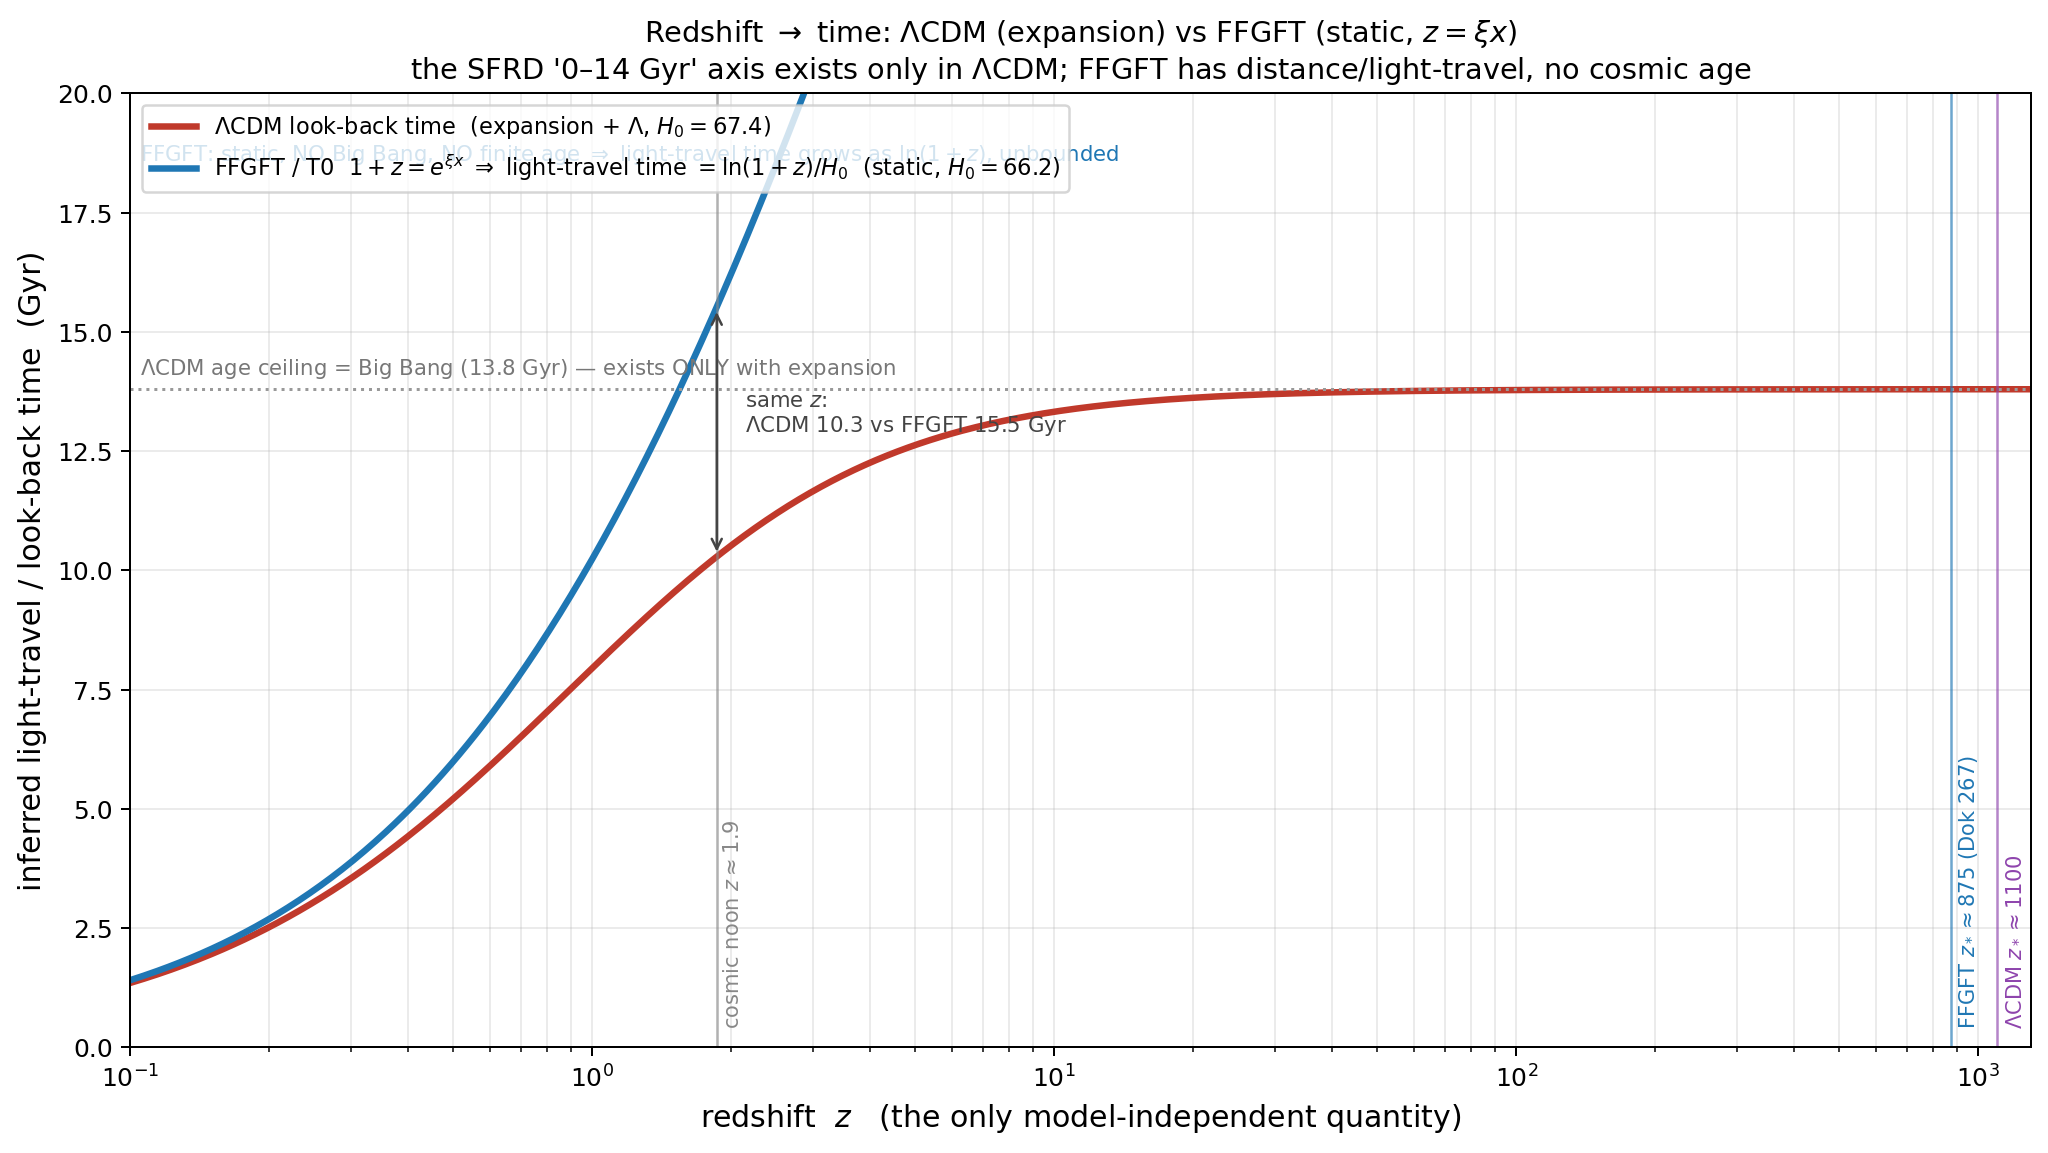
\includegraphics[width=0.96\textwidth]{../fig/280_z_time_ffgft.png}
  \caption{Rotverschiebung $\to$ Zeit ist modellabhängig. $\Lambda$CDM-Lookback
  (rot, Expansion $+\Lambda$) saturiert bei der Urknall-Decke $13{,}8$\,Gyr;
  FFGFT (blau, statisch, $1+z=e^{\xi x}$) liefert eine unbeschränkte Lichtlaufzeit
  $\ln(1+z)/H_0$ ohne Urknall. Bei \enquote{cosmic noon} ($z\approx1{,}9$):
  $\Lambda$CDM $10{,}3$ vs.\ FFGFT $15{,}5$\,Gyr. Rekombination: $\Lambda$CDM
  $z_*\approx1100$, FFGFT $z_*\approx875$ (Dok.~267).}
\end{figure}

\textbf{Folgerung:} Eine Auftragung \enquote{Sternentstehungsrate über kosmische
Zeit 0--14\,Gyr} (Lilly--Madau) ist intrinsisch ein $\Lambda$CDM-Akt. In FFGFT
existiert keine kosmische Zeitachse -- nur Distanz bzw.\ Lichtlaufzeit. Die
Datenpunkte $(z,\text{SFRD})$ bleiben gültig; ihre Platzierung auf einer
$0$--$14$-Gyr-Achse \emph{ist} bereits die Übertragung auf das expandierende Bild.

% ============================================================
\section{Wie passen die Messdaten? -- die kosmologische Entartung}
% ============================================================

Dok.~267 zeigt die zentrale Tatsache: FFGFT und $\Lambda$CDM sind auf den
Standard-Tests \emph{beobachtungs-entartet}. Was eine bestimmte $z(d)$-Relation
erzeugt, erzeugt dieselben Flüsse, Winkel und Zeitdehnungen.

\begin{itemize}
  \item \textbf{Supernova-Zeitdilatation:} Ferne SN~Ia laufen gedehnt ab,
        $b\approx1$ (DES: $b=1{,}003\pm0{,}011$). Die fraktale Wegverlängerung
        dehnt Wellenlänge \emph{und} Pulsdauer im selben Verhältnis $\Rightarrow b=1$.
        Der Test schließt nur \emph{nicht-dilatierendes} tired-light ($b=0$) aus --
        FFGFT sagt $b=1$ voraus und ist nicht betroffen.
  \item \textbf{BAO-Winkelskalen:} Die nicht-lineare zeitliche Rekursion krümmt
        $z(d)$ wie eine beschleunigte Expansion $\Rightarrow$ dieselben Winkel.
        Vorbehalt P20: BAO nutzt $D_M/r_s$ mit $r_s$ aus $\Lambda$CDM -- Modell
        gegen Modell.
  \item \textbf{CMB-Peaks:} Beide reproduzieren die Peakstruktur; $\xi$ spielt für
        die Peaks keine Rolle; beide gleich zirkulär (Dok.~267/268).
  \item \textbf{Lilly--Madau / SFRD:} Das $z$-Raum-Signal (Anstieg bis $z\sim2$,
        Abfall) ist modellunabhängig und in FFGFT astrophysikalische
        Galaxienentwicklung über die Lichtlaufzeit. Die SFRD-\emph{Werte}
        (M$_\odot$/yr/Mpc$^3$) sind jedoch doppelt $\Lambda$CDM-abgeleitet --
        über die Leuchtkraftdistanz $d_L(z)$ und das mitbewegte Volumen. Ein fairer
        FFGFT-Test rechnet sie mit $d(z)$ und Volumen aus $1+z=e^{\xi x}$ neu.
\end{itemize}

\textbf{Ehrliche Lage:} Die Entartung schneidet in beide Richtungen. Die Daten
\emph{passen} zu FFGFT (keine falsche Vorhersage, achromatisch wie beobachtet),
aber sie \emph{erzwingen} es nicht. Der Fall für FFGFT ruht damit auf
\emph{Sparsamkeit} (kein $\Lambda$, keine dunkle Energie, keine $H_0$-Spannung --
Dok.~064) und auf der Ableitung der Konstanten aus $\xi$ -- nicht auf einem
einzelnen Diskriminator.

% ============================================================
\section{Kein Urknall -- die Entwicklungsrichtung kehrt um}
% ============================================================

FFGFT kennt keinen Urknall. Der scheinbare Hochrotverschiebungs-\enquote{Anfang} --
der Abfall der SFRD und das vermeintliche Einsetzen der ersten Galaxien bei
$z\sim14$ -- ist in FFGFT \emph{kein} zeitlicher Beginn, sondern ein
\emph{geometrischer Umkehrpunkt} (Dok.~263).

Die beobachtete Größe ist die kumulierte fraktale Wegverlängerung
$z_{\text{obs}} = (L_{\text{eff}}-d)/d$ (Dok.~026/263). Für kleine $z$ ist sie
linear, $z(d) = \kappa\,d$ mit $\kappa = E_H/(\hbar c)$ -- die Steigung, die
$\Lambda$CDM \enquote{$H_0$} tauft. Nahe der kosmologischen Maximalskala $R_H$
besitzt die $z(d)$-Kurve jedoch einen \emph{Extremwert}: FFGFT \emph{berechnet} dort
$z_*\approx 875$ (Dok.~267, Referenzwert; Vorbehalt P20) -- dieselbe Fläche, die
$\Lambda$CDM als Rekombination/Entkopplung bei $z\approx 1089$ liest. Der
ΛCDM-Wert $1089$ ist also nur die Expansionsdeutung; der FFGFT-eigene Wert ist
$875$, \emph{nicht} $1100$. \emph{Jenseits} von $R_H$ gilt $z\to\infty$ -- ohne
Teilchenhorizont und ohne Urknall.

\textbf{Was ist $z_*$ aus FFGFT-Sicht?} Es ist \emph{keine} Rekombinationszeit. FFGFT
hat keine heiße Frühphase, kein Photon-Baryon-Plasma, keine Entkopplung. Die CMB ist
der \emph{stationäre Quanten-Grundzustand} des $\Phi$-Feldes (Dok.~025), und ihre
Akustikpeaks sind diskrete T$^4$-\emph{Gitterresonanzen} (analog zu Emissionslinien
eines Atoms oder Phonon-Dispersionen im Kristall) -- \emph{nicht} eingefrorene
Schallwellen eines Urplasmas. Der Zahlenwert selbst ist ein \emph{geometrisches
Verhältnis} (Dok.~267):
\[
  z_* \approx \left(\frac{\lambda_e}{L_0}\right)^{1/\ln(1/\xi)} \approx 875,
\]
mit der reduzierten Compton-Wellenlänge $\lambda_e$ und der Sub-Planck-Länge
$L_0=\xi\,\ell_P$ -- also eine \emph{Resonanz- bzw.\ Strukturskala} des T$^4$-Gitters,
kein thermisches Ereignis in der Zeit. (Vorbehalt P20: der Exponent $1/\ln(1/\xi)$ ist
noch nicht aus der T$^4$-Geometrie hergeleitet; $z_*$ ist derzeit ein Referenzwert in
der richtigen Größenordnung, kein abgeleitetes FFGFT-Resultat.)

Damit \textbf{kehrt sich die scheinbare Entwicklungsrichtung an der Maximalskala um}:
Was $\Lambda$CDM als \enquote{früher = schnellere Entwicklung bis zu einem Anfang}
liest, ist in FFGFT die Annäherung an den geometrischen Extremwert nahe $R_H$. Der
Hochrotverschiebungs-Abfall der SFRD ist daher die Annäherung an diesen Umkehrpunkt,
\emph{kein} Beginn. $H_0$ ist dabei emergent, kein fundamentaler Parameter -- in der
kompakten $T^4$-Form gibt es überhaupt kein $H_0$ (Dok.~263).

Symmetrisch offen bleibt allein die Vorwärts-Herleitung des Exponenten $41/4$ aus
$\xi$ (Dok.~190~P20) -- sie fehlt jedem Rahmen, nicht nur FFGFT.

\section*{Status}

Statische Rotverschiebung $1+z=e^{\xi x}$: \emph{Kern} (Dok.~064/026).
Achromatie: \emph{korrigiert/etabliert} (FE-Simulation; Dok.~190~K6).
$z\to$Zeit als $\Lambda$CDM-Übertragung und kosmologische Entartung:
\emph{etabliert} (Dok.~267). Status durchgehend nach Dok.~190.

\end{document}
